\documentclass[11pt,letterpaper]{article}
\pagestyle{plain}
\usepackage{amsmath}
\usepackage{amssymb}
\usepackage[utf8]{inputenc}
\usepackage{times}
\usepackage{hyperref}
\usepackage{graphicx}
\usepackage{wrapfig}
\usepackage{listings}
\usepackage[usenames,dvipsnames]{xcolor}
\usepackage{setspace}
\usepackage{python_syntax}
\usepackage{natbib}
\usepackage{bibentry}
\usepackage{todonotes}
\usepackage{url}
\usepackage[compact]{titlesec}
\usepackage{enumitem}
\usepackage[
top    = 1in,
bottom = 1in,
left   = 1in,
right  = 1in]{geometry}
\linespread{0.92} % NSF allows up to 6 lines per inch.  
\def\UrlFont{\em} % Italicize all URLs.  
\frenchspacing
\setlist{nolistsep} % or \setlist{noitemsep} to leave space around whole list

\begin{document}

\section{Introduction}
Scientists construct quantitative models to explain observations about natural systems in a coherent and rigorous manner. Today, as the number of models and the quantity of empirical data increases, scientists face a grand challenge: efficiently discovering relevant models and characterizing their validity against a continually growing body of available evidence. 

A new model is typically proposed by publishing a description of how it works along with an argument justifying its utility to some targeted scientific community. This argument is made in words, accompanied by a few relevant equations and figures, and judged by peer review. Ideally, reviewers determine whether the model's predictions are consistent with all available and relevant data and compare performance against previously published models. This is increasingly difficult; although authors are may refer to relevant experimental data and review the literature, these citations are incomplete and biased, in that authors will focus on data favorable to their models, or compare them to implausibly simple null hypotheses.

If modeling papers contained figures a) highlighting accordance with all related experiments and b) comparing performance to all related models, publications would be encyclopedic with their main points obscured. A strength of model publication is focused description of how a model works and its conceptual and technical advances. A weakness, however, is that evaluating the scope and validity of a model is intractable using a publication alone. Publications tell us \textbf{how} a model works but are less effective at reporting \textbf{which} goals it achieves and \textbf{how well} it achieves them. This problem is exacerbated as future data is gathered. Although model validity may change in light of new data, there is no systematic process in biology today for re-evaluating existing models. Although new data and its theoretical implications may propagate informally through a scientific community or appear in periodic reviews, the original publications -- a resource of first resort for new scientists and onlookers -- are cited "as-is'' in perpetuity. 	

The central problem discussed here: the process of model validation is not rigorous, comprehensive, or ongoing. This hampers experimental prediction, simultaneous comparison of models, and identification of outstanding research problems. To overcome these obstacles, we propose formalizing the model validation process by creating software and associated cyberinfrastructure dedicated to the systemization of scientific model validation.  This validation framework will exist in parallel to publication, allowing the latter to focus on answering \textbf{how}, while the former can answer \textbf{how well}. 

\subsection{Existing Efforts}\label{sec:existing_efforts}
There are several facilities developed for data and model sharing in biology, but few if any facilitate evaluation of models against data.  For example, the Collaborative Research In Computational Neuroscience (CRCNS) data-sharing website \cite{crcns_url}, and the Open Source Brain (OSB) repository \cite{osb_url} are facilities for data and model sharing in neuroscience, respectively.  The CRCNS website hosts several excellent data sets of relevance to computational models; however, the data is not organized or annotated in a way that permits systematic model validation.  The OSB is focused on model description and reliable execution; however, it lacks a means to test models. We aims to bridge such resources, strengthening each in turn.

Related efforts in the machine learning community promote model development and validation against publicly-available datasets.  Kaggle \cite{kaggle_url} drives model development by organizing competitions where training data is made public and competitors submit competing algorithms, compared automatically by cross-validated accuracy on an unrevealed test set. The success of Kaggle \cite{carpenter_may_2011}\todo{A more recent reference might be better since Kaggle has grown a lot since 2011, but this reference is in Science and other ones I saw are in trade magazines.} shows that open competitions are effective, and that this paradigm of "modeling as a competition'' attracts data scientists across traditional discipline boundaries. However, models developed in this way fit only a few general cases in machine learning: classification, regression, and clustering. Validation criteria are straightforward in these domains. Discipline-specific competitions for biology have also resulted in technical advances.  The quantitative single neuron modeling competition \cite{jolivet_quantitative_2008} has helped us understand the complexity-accuracy tradeoff among reduced models of excitable membranes; the "Hopfield'' challenge \cite{hopfield_what_2000} famously illustrated the challenges of identification facing computational neuroscience; the Diadem challenge is advancing the art of neurite reconstruction \cite{diadem_url}; and examples from other subfields of biology abound \cite{dream_url}. Our challenge is to develop a general framework in support of distributed data-driven model validation workflows, but where validation criteria may be complex and discipline-specific. Initially, we will be focus on validation challenges in the biological sciences, particularly neuroscience. 

\section{Outcomes and Products}
Our framework is based on simple validation tests that compute agreement between a model execution result and an experimental observation. Model validity can be identified with the collection of tests passed by the model. This methodology is inspired by the ubiquitous "unit testing" practice of software engineering. A unit test evaluates whether a portion of a computer program (often a single function) meets a simple correctness criterion. A suite of such tests covering desired program behavior validates overall program functionality, and isolates specific causes of failures. Developers often write unit tests before writing the program itself, following a methodology called test-driven development (TDD) \cite{beck2002}\todo{Fix reference}. TDD asserts that a suite of unit tests serve as a program's specification, guiding its development. This allows developers to measure progress simply by looking at the proportion of tests that pass at any point in development. When modifications are made, developers can ensure that existing functionality is maintained by ensuring that all previously passed tests continue to do so.  The success of unit testing and TDD in practice suggests that validation testing is a practical solution to model validation. 

\subsection{Example}\todo{Is this whole section useful?} What might a scientific model validation test look like?  We begin with a neuroscience example, derived from experiments where a stimulus is delivered to a neuron, in the form of somatically injected current, while the somatic membrane potential of that cell is recorded and stored.  A model claiming to capture the membrane potential dynamics of this cell type might be validated in several ways; one simple test of that claim would check for correspondence between the distributions of action potential counts produced by the model and the data, respectively. This test would ask a candidate model to produce a prediction for each provided input current and then check whether each prediction agrees with the data for that input current.  The measure and degree of agreement are specified by the test creator.  For example, model action potential counts that, for each value of input current, fall with the 95\% confidence interval of the empirical data distribution might constitute a passed test. This choice is made explicit in the test specification, so modelers need not guess which criteria testers may be using for validation.

\subsection{Community Workflow}\todo{Maybe this section should be moved to the end of the introduction}
Unit tests are produced by the community of developers involved in the development of a program. Correspondingly, members of a scientific community can collaboratively produce suites of validation tests in common source code repositories. Each test specifies the model requirements, and provides a procedure for determining whether a candidate model (the input to the test) is consistent with a particular summary of experimental observations (the parameters of the test). Model performance on a collaboratively curated suite of validation tests can serve as justification of claims regarding the model's validity as a description of the scientific system characterized by the test suite. This workflow continuously produces a summary of the field indicating which models are capable of taking each test, i.e. whether the test falls within the model's scope, and for each capable model, how well it performed, i.e. its validity.  Model usefulness becomes a function of the weight given to each test, determined per investigator or by community consensus. This test-driven scientific workflow leverages the desire of modelers to promote their models' virtues -- test suites represent clear \emph{challenges}, issued by experimentalists to the community, and passed tests certify success for the modelers. As more data is gathered and test suites are refined, past models can be tested continuously againt current empirical knowledge, in a fully-automated manner because the interface between tests and models is fixed.  

\subsection{\textit{SciUnit}: A Simple Validation Testing Framework}\todo{Maybe this section should be the start of "Outcomes and Products"}
Conceptual and practical simplicity -- the absence of "heavy-lifting'' -- is an essential requirement for community participation. Our design does not require the release of raw data or storage in standard formats. Instead, salient aspects of the data are abstracted away behind a test definition. Similarly, implementation details of a model (e.g. its programming language) need not be public or standardized -- the implementation must simply be wrapped to expose a standardized interface, so that tests can access model capabilities. Each community can collaboratively specify model interfaces capturing high-level operations of their preferred modeling formalisms. Existing modeling standards (e.g. NeuroML \cite{neuroml_url,gleeson_neuroml:_2010}) and interface definition languages (IDLs) \cite{bachmann2008}\todo{Fix reference} are leveraged to simplify this process. \textbf{Thus, the first product of this proposal is an object-oriented validation testing framework called \textit{SciUnit}, written in Python, that makes test construction (from data) and test-driven model execution easy and flexible.} 

\begin{wrapfigure}[18]{r}{0.5\textwidth}
\centering
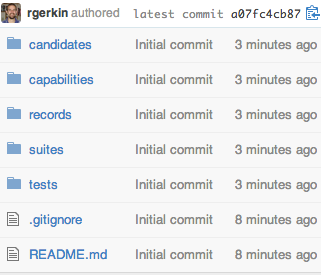
\includegraphics[scale=0.7]{scidash_github.png}
\label{fig:scidash_repo}
\caption{A \textit{SciDash} repository on GitHub}
\end{wrapfigure}
\leavevmode
\todo{Update this figure when SciDash repo structure is finalized.}    

\subsection{\textit{SciDash}: A Community Web Portal}
This framework is most effective when the current state of a research area is represented by a collection of tests and models. This requires coordination among research groups, so community-oriented cyberinfrastructure to support test suite creation and summarization, building upon \textit{SciUnit}, is essentiall. We propose a service, called \textit{SciDash}, utilizing existing infrastructure for coordinated development of software repositories, focusing on GitHub \cite{github_url} \cite{ram_git_2013}. A suite of related tests will be contained in a GitHub repository with a stereotyped high-level structure that allows the \textit{SciDash} web portal to discover, index and summarize it on an ongoing basis (Fig. \ref{fig:scidash_repo}). The portal, a web application written using the pythonic Django framework \cite{django_url} will serve as a central location where scientists can discover relevant test suites, determine test requirements, and summarize the results of test execution on submitted models. Test results can be visualized as a "record matrix" composed of large numbers of model/test combinations (Table \ref{table:record_matrix} provides a toy example).  Each row in this matrix will contain results for all tests taken by one model and would serve as clear evidence of that model's scope and validity.  Models, tests, and records will be stored on GitHub, pointed to by hyperlinks in the record matrix. \textit{SciDash} will serve as a public record of competition among models, facilitating and encouraging data-driven development among modelers. \textbf{Thus, the second product of this proposal is a web application called \textit{SciDash}, whose back-end can index test suite repositories collaboratively developed on GitHub, and whose front-end offers users a simple environment for discovery and evaluation of models, tests, and results.}  

\subsection{\textit{NeuroUnit}: A Suite of Tests for Neurophysiology}\label{sec:neurounit}
To demonstrate the utility of these tools, an initial case study must be conducted. Because we have substantial experimental and computational neurophysiology training and expertise, we target the work toward this domain. By using machine-readable models from the Open Source Brain repository, and corresponding machine-readable data from resources like The NeuroElectro Project\todo{URL via citation}, our efforts will produce a body of useful tests that also serve as a demonstration of the test-driven workflow that other areas in the biological sciences can leverage.  \textbf{The third product of this proposal is \textit{NeuroUnit}, a large suite of data-driven tests and model interfaces for a representative set of canonical neurophysiology models, all publicly available. A case study examining the implementation of \textit{NeuroUnit} will inform development of domain specific test-suites in other biology sub-fields.}

\section{Preliminary Activities}
We have developed most of the core testing framework, \textit{SciUnit}, under a free, open-source license at the project development repository \cite{sciunit_url}.  

\subsection{\textit{SciUnit} Implementation} We implemented \textit{SciUnit} using the Python programming language \cite{python} due to its widespread adoption across the quantitative sciences. Python also supports interoperability with other major languages used within science, including C, R \cite{r_url}, and MATLAB \cite{matlab_url}. The functionality described below could also be readily translated into any programming language with comparable facilities.

\subsection{Validation Tests}\label{sec:validation_tests} 
Testing in \textit{SciUnit} proceeds in three phases (Figure \ref{fig:sciunit_flowchart}): 
\begin{enumerate}
\item Capability Checking: The test checks to see that the model is capable of taking the test; i.e., that it exposes the needed functionality for the execution phase to proceed.
\item Test Execution: The model is executed to produce the model output by interacting with its supported capabilities.  If the model is described according to a standard specification, e.g. NeuroML, this corresponds to loading it into a supported simulator and executing it. 
\item Output Validation: The model output is compared to empirical data to determine whether the model passes.  This comparison can be of several types: for deterministic models, we may extract a matching quantile from a data distribution; for stochastic models, we may compute a measure of agreement between model output and data distributions, e.g. the Kolmogorov-Smirnov statistic.  Validation is ultimately pass/fail, but in some cases the result generated in this phase also includes a continuous statistic so that models can be ranked based on their test results in a more fine-grained manner.   
\end{enumerate}

\begin{wrapfigure}{r}{0.42\textwidth}
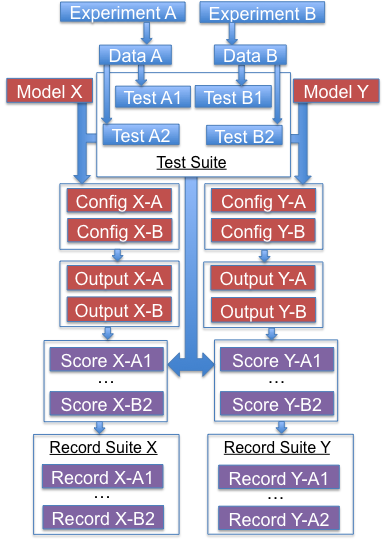
\includegraphics[scale=0.5]{sciunit_flowchart.png}
\caption{Workflow in \textit{SciUnit}. \scriptsize{i) Each experiment generates data, ii) From each set of data, many validation tests can be generated from test families (not shown); an ensemble of tests (from data within or across experiments) forms a test suite.  iii) Tests enumerate capabilities required for models to take them, and provide metadata used to configure models for execution.  iv) Model execution output is checked against test rules to produce a score.  Some test scores are not indicated here (…) for clarity.  v) The score establishes a validation record for that model+test combination.  An ensemble of records for one model is a record suite, and summarizes the scope and validity of the model.}}
\label{fig:sciunit_flowchart}
\end{wrapfigure}

A validation test in SciUnit is an instance of a Python class implementing the \verb|sciunit.Test| interface. Classes that implement this interface must contain a \verb|run_test| method that receives a model as input and produces a normalized score as output. The capabilities that the model must possess in order for the test to operate correctly are given using the \verb|required_capabilities| attribute. In many cases, several tests will have a similar form, differing only by a choice of parameters or by association with a particular dataset. Such parameterized test families correspond to subclasses of sciunit.Test that take the needed parameters as constructor arguments. 

In Figure \ref{fig:rate_test}, the \verb|RateTest| class implements a parameterized family of tests that compare the output firing rate (action potentials per second) of a neuronal model, driven by a given somatic input current, to an empirically measured mean and standard deviation of the rate derived from a set of replicated experiments. The test produces a boolean score indicating agreement within one standard deviation of the empirical mean. The input currents, mean, and standard deviation are provided as constructor arguments on line 2 (constructors are named \verb|__init__| in Python.) On lines 5-8, the required capabilities are listed: the model must be able to take a current as input and produce firing rates as output. These capabilities are used in the \verb|run_test| method, on lines 11 and 12 respectively, to execute the model against the provided current. The resulting firing rate is compared to the empirical mean and standard deviation on line 15 and a boolean score is produced on lines 16-20. In addition to the boolean value itself, the score also contains metadata that may be useful to scientists wishing to examine the result in detail. In this example, we save the model's output rate and the provided mean and standard deviation alongside the result, by specifying the \verb|related_data| parameter.
\todo{Check line numbers above.}  

To create a validation test, a scientist instantiates the RateTest class with a particular mean, standard deviation and input current (I, not shown):
\\
\\
\verb|CA1_cell_rate_test = RateTest(mean=18.0, std=40.0, input_current=I)|
\\

The test is then executed against a model instance (described below), using the \verb|sciunit.run| function:
\\
\\
\verb|score = sciunit.run(CA1_cell_rate_test, CA1_cell_model)|
\\

The \verb|sciunit.run| function operates in three phases, implementing the abstractions at the beginning of section \ref{sec:validation_tests}:
\begin{enumerate}
\item Capability Checking: The model is verified as capable of taking the test by checking each capability in the test's \verb|required_capabilities| attribute.
\item Test Execution: The test's \verb|run_test| method is called to execute the model and cache output.
\item Output Validation: \verb|run_test| returns an instance of a \verb|sciunit.Score| subclass containing a goodness-of-fit metric between the model output and the data used to instantiate the test.
\end{enumerate}

Any errors that occur during this process are reported by raising an appropriate exception.

\subsection{Test Suites}
A test suite is a collection of tests designed to validate a model against several mutually coherent requirements:
\\
\\
\verb|spike_tests = sciunit.TestSuite([SpikeWidthTest, SpikeHeightTest])|
\\

When a test suite is executed against a model, it produces summary data that can be shown on the console or visualized by other tools, such as the web application described in the next section.

A test suite can also be used to compare multiple models (described below), producing a table as in Table \ref{table:record_matrix}.

\begin{figure}
\caption{A single neuron firing rate test implemented in \textit{SciUnit}}
\label{fig:rate_test}
\begin{python}
class RateTest(sciunit.Test):
	def __init__(self, mean, std, input_current):
		self.mean, self.std, self.input_current = \
		mean, std, input_current
	
	required_capabilities = (
		neurounit.Capabilities.ReceivesCurrent,
		neurounit.Capabilities.ProducesFiringRate
	)
	
	def run_test(self, model):
		model.set_current(self.input_current) 
		# Implementation guaranteed by capability check.  
		rate = model.get_firing_rate()
		
		mean, std = self.mean, self.std
		result = (mean - std) <= rate <= (mean - std)
		return sciunit.scores.BooleanScore(result, related_data={
			"rate": rate,
			"mean": mean,
			"std": std
		})
\end{python}
\end{figure}

\subsection{Candidates and Capabilities}
A candidate is the entity to be tested.  In practice, this will almost always provide an implementation for a particular scientific model, so candidate and model can be used interchangeably; we distinguish them allow for the possibility of testing datasets against each other as well.  For clarity, we will refer to candidates as models herein.  In our framework, a model is represented by an instance of a class inheriting from \verb|sciunit.Candidate|, provided by the framework.  In many cases, models can be grouped into parameterized model families, as with tests. These parameters correspond to parameters passed to a subclass constructor.
In order for a model to be tested, it must have certain capabilities that the test requires.  That is, the model must be capable of taking certain kinds of input and generating certain kinds of output that the test will use to evaluate its quality.  A capability is a contract that guarantees that a model is able to produce results of a particular form. We model capabilities as Python classes containing unimplemented methods. In other object-oriented languages, this would correspond to an interface or an abstract class.  
Let us consider the capabilities of a model publicly available on the Open Source Brain website \cite{osb_ca1_url}.  In the experiment being modeled, recorded data consists of somatic membrane potential of a pyramidal neuron from area CA1 of the hippocampus, and the stimulus consists of somatically-injected current.  This somatic membrane potential includes action potentials, the rate of which is known in neurophysiology as the "firing rate".  The following are some examples of corresponding model capabilities:  

A wide variety of capabilities (as in example above) would be enumerated to span the modeling formalisms in use by a community. In the simple example we present here, these three capabilities suffice.  As they are domain-specific (to neuroscience), we place them not in \textit{SciUnit} itself but in \textit{NeuroUnit} in the module \verb|neurounit.capabilities|.  In contrast, \verb|sciunit.capabilities| contains only domain-independent model capabilities, e.g. \verb|TimeIntegrable| (can this model be integrated over time?)

A model is represented by an instance of a class inheriting from \verb|sciunit.Candidate|.  In the examples below, the CA1 cell model and Purkinje cell model families each exhibit different capabilities, which determine which tests are within their scope.  These differences arise because the researchers who implemented the model did so at different levels of detail.  In particular, the Purkinje cell was modeled with individual dendritic compartments, so there is an associated dendritic membrane potential. 

\begin{figure}
\caption{A candidate class corresponding to a CA1 Pyramidal Cell model from Open Source Brain}
\label{fig:ca1_model}
\begin{python}
class CA1PyramidalCellModel(candidates.NeuroConstructModel,
				            capabilities.ReceivesCurrent):
	"""CA1 Pyramidal Cell model from /neuroConstruct/osb/hippocampus/
	CA1_pyramidal_neuron/CA1PyramidalCell"""
	def __init__(self,**kwargs):
		# Put any other initialization here.
		project_path = os.path.join(candidates.putils.OSB_MODELS,
									"hippocampus",
									"CA1_pyramidal_neuron",
									"CA1PyramidalCell",
									"neuroConstruct")
		candidates.NeuroConstructModel.__init__(self,project_path,**kwargs)
		super(CA1PyramidalCellModel,self).__init__(**kwargs)
\end{python}
\end{figure}

In each example, the model produces a firing rate after being provided a current.  This is implemented with multiple inheritance, so that each model expresses methods (such as \verb|set_current|) that override (and implement) the abstract method provided in the corresponding capability classes.  Any capability that the model inherits must have all if its associated methods implemented.  Failure to do so will result in a \verb|NotImplementedError|, which indicates that the model scope was less than what was claimed.  

The model class is initialized with parameters (\verb|i_leak| in the case of the CA1 cell model) to produce a model instance, which is essentially a model with specified parameters.  A tester can specify that model instances taking a test should be initialized with particular parameters, or ranges of parameters. The writer of a test can provide as many or as few of these specifications as she feels are needed to instantiate models capable of passing the test.  These specifcations may reflect important experiment context or metadata, such as known values of key system parameters, or the contents of a pharmacalogical milieu.  In the RateTest above, the tester might specify the mean input resistance of recorded neurons; while this value may not be of interest in itself, it may be required to initialize a model instance capable of passing the test.  The specification could also include a subset of the data of interest, which the model instance can use for training prior to a testing phase.  Figure \ref{fig:sciunit_flowchart} illustrates the testing workflow, and Table \ref{table:glossary} provides definitions for terms used here.  
 
\begin{table}[h]\footnotesize
\caption{Glossary of Terms}
\label{table:glossary}
\begin{tabular}{| c | p{13cm} |}
\hline
Data & The measurements yielded by an experiment.\\ \hline  
Model & An executable function that aims to explain, reproduce, or predict experimental data.  More generally, a candidate.\\ \hline
Model Family & A class that generates a set of related model instances. Each model instance from one family differs according to the set of parameters (corresponding to a particular experimental design, or set of training data) with which it was initialized.\\ \hline  
Validation	 & The process of assessing the agreement between model output and experimental data.\\ \hline
(Validation) Test & A function that executes a model and scores the model’s output against a summary of experimental data. One experiment can inform the development of many tests.\\ \hline  
Test Family & A class that generates a set of related test instances.  Test instances from within one family differ only quantitatively, according to the data used to initialize them.  All tests from one family attempt to validate the same property of a model.\\ \hline
Test Suite & A collection of tests, each of which attempts to validate a different property of a model.\\ \hline  
Score & A value summarizing the performance of a model on a test. This can be a measure of the goodness of fit between model output and experimental data.\\ \hline
Scope & A list of tests that a model is eligible to take, indicating the range of experimental data that the model might be able to explain or replicate.\\ \hline
Capability & 	A contract that states that a model is able to produce results of a particular form. For example, a Hodgkin-Huxley neuron model is capable of producing a membrane potential time-series, whereas a model without a notion of voltage is not.\\ \hline
Record & An indication of the test score achieved by a model, along with any initialization conditions.\\ \hline
Record Suite & A list of records associated with a model.  This summarizes the scope and validity of the model.\\ \hline  
\end{tabular}
\end{table}

\subsection{\textit{SciDash} Development}
We have also begun work on the \textit{SciDash} web portal, which will serve to aggregate tests and their results for the scientific community. A development version is currently live \cite{scidash_url}.  We have populated it with the models and tests from the educational illustration in Table \ref{table:record_matrix}.  This application has several key features.  \textbf{First}, it will provide a "dashboard" view of the state of a field by displaying a matrix of records for selected model/test combinations.  By designing the site with modern javascript-based data visualization libraries, users will be able to filter this matrix quickly to obtain the relevant subset of models and tests most relevant to their scientific questions.  \textbf{Second}, each record will link to a Sage notebook worksheet displaying line-by-line the code that was executed and any intermediate output statements.  Sage \cite{stein_sage:_2005,sage_url} is free open-source mathematics software heavily funded by NSF, based on a Python environment.  The Sage notebook \cite{sagenb_url} is a web application whose "worksheets" offer a means to publish and collaborate on a block of code, and to view its numerical and graphical outputs.  While Sage was written for Python, the notebook also supports the execution of code and visualization of outputs from other programming languages, making possible worksheets based on MATLAB, Mathematica, and other popular environments for modeling.  \textbf{Third}, a community-moderated comment section will allow test-makers and test-takers to discuss issues associated with each record.  Thus, disagreements about the appropriateness of a test can be openly aired and in many cases resolved.  Rather than require special login credentials, we support open authentication via existing web portals (Google, Yahoo, Twitter, etc.), lowering the barrier to participation.  The \textit{SciDash} backend will consist of a MySQL relational database and XML files.  
\todo{Replace discussion of Sage with use of github for SciDash repositories.}  

\section{Research and Development Plan}
In order to 1) accelerate development and testing of the framework and 2) populate it with models and tests, we will focus during the period of this grant on one scientific discipline (neurophysiology), without compromising generalizability to other fields. This will allow us to get rapid feedback from an experimental community the authors are familiar with as we iterate through the software development cycle.  

\subsection{Leverage of existing resources for the development of \textit{NeuroUnit}}
Here we describe standard tools in neuroinformatics that we have adopted to develop \textit{NeuroUnit} \cite{neurounit_url} with the neurophysiology community in mind.  

\subsubsection{Candidates from NeuroML Models}
NeuroML is a standardized model description language for neuroscience \cite{gleeson_neuroml:_2010}. It permits most neurophysiological and neuroanatomical models to be described in a simulation-independent fashion, and these models can be run in any of a number of popular simulators due to the programmatic inter-conversion capabilities of the NeuroML API.  Because NeuroML is an XML specification, which can be both validated for correctness and queried for model properties and components, it is ideal for model sharing and curation, as well as for answering what and how in a machine-readable manner.  

To this end \textit{NeuroUnit} offers a \verb|sciunit.Candidate| subclass called \verb|NeuroConstructModel|. NeuroConstruct \cite{neuroconstruct_url,gleeson_neuroconstruct:_2007} is a simulation manager that starts with NeuroML models and then simulates them in any of the conventional simulators listed above. \verb|NeuroConstructModel| is instantiated with the path to any NeuroML model created in or imported into NeuroConstruct.  Because the family of all models that can be described by NeuroML is vast, the \verb|NeuroConstructModel| class makes very limited assumptions about the candidate models: that they are runnable, and that at least one compartment generates a membrane potential. \verb|NeuroConstructModel| is then subclassed to test specific NeuroML models. 

The Open Source Brain project (OSB, \cite{osb_url}) curates many such models. In contrast to previous curation efforts such as ModelDB \cite{modeldb_url,hines_modeldb:_2004}), OSB projects have been converted from their native format into NeuroML, and run on all major simulators for neurons and networks, such as NEURON, Genesis, PyNN, Moose, and others. Thus, OSB models are effectively guaranteed to be runnable.  In addition, the degree of concordance between model output (beginning with the NeuroML description) and reference output (from the original source files) is reported for each model, and is generally near perfect.  Thus, OSB is an excellent source of models that, in addition to being open source, are described completely enough to make validation possible.   The hippocampal CA1 pyramidal cell is represented in several OSB models, and we demonstrate testing using a \verb|CA1PyramidalCellModel| class (Figure \ref{fig:ca1_model}), deriving from \verb|NeuroConstructModel|.  All OSB models, and indeed any NeuroML model, can be tested similarly.  Working together with OSB is part of our \textbf{first collaboration}, and our integration efforts can be publicly tracked in our fork of the neuroConstruct code repository \cite{neuroconstruct_rgerkin_url}.  

Although they span a range of scales, and regardless of their original implementation, all OSB models are formally described using NeuroML, as are each of the model components and sub-components, such as cells, ion channels, calcium stores, etc.  These models are regularly executed on OSB servers to ensure that, as they are updated, their output is consistent with previous versions.  Therefore, OSB can confirm that they work, and linked journal articles, and on site wiki, and inspection of the native code or NeuroML itself can establish how they work. However, currently there is no mechanism for establishing how well they work, i.e. how well the models perform at explaining data.  \textit{SciUnit} will fill this gap by providing OSB (and the biology community in general) with a means to assess models using data-driven tests in the \textit{NeuroUnit} library.  Consequently, researchers will be able to see not only what is being modeled and how -- as OSB currently facilitates -- but also how well model output conforms to measured neurophysiological properties. OSB models will be tested using the \textit{SciUnit} framework, utilizing \textit{NeuroUnit} tests of our own design as well as those contributed by the community.  A similar process can be used to apply \textit{SciUnit} to other biology sub-disciplines using corresponding community repositories of models from those disciplines.

\subsubsection{Capabilities from NeuroTools}
NeuroTools \cite{neuralensemble_url} is a collection of tools written in Python to support all tasks associated with a neural simulation project and which are not handled by the simulation engine.  Specifically, it permits the extraction and analysis of simulation output, such as membrane potential time series, spike trains, etc. NeuroTools is an open source and actively developed projecs, and represent reliable libraries on which neurophysiology tests can be based. 

We use these libraries to implement \textit{SciUnit} Capabilities in \textit{NeuroUnit} (Figure \ref{fig:neurounit_example}).  For example, a NeuroTools \verb|AnalogSignal| object (e.g. a membrane potential time series) has threshold detection method that returns a NeuroTools \verb|SpikeTrain| object.  A \textit{NeuroUnit} \verb|HasSpikeTrain| Capability requires that the method getSpikeTrain be implemented.  While one could implement this in any number of ways, a NeuroConstructModel does so by making \verb|getSpikeTrain| wrap \verb|AnalogSignal.threshold_detection|.  This is one of many examples in which NeuroTools objects are exchanged between \verb|NeuroConstructModel| methods.  This greatly simplifies test writing, since many basic properties of model output are obtained trivially by using NeuroTools object methods, and these NeuroTools objects are easily extracted from model output using candidates derived from the \verb|NeuroConstructModel| base class.  This is possible because NeuroConstruct already implements the creation of NeuroTools objects from model output.  

\subsubsection{Reference Data for Tests from NeuroElectro}
Answering how well requires validation testing against data. The NeuroElectro project \cite{neuroelectro_url} is an effort to curate all published single cell neurophysiology data \cite{tripathy_neuroelectro:_2012}.  Currently, up to 27 electrophysiological properties are reported for 93 cell types, spanning over 2000 single pieces of published data extracted from article tables.  \textit{NeuroUnit} makes it easy to construct Tests that use reported values on neuroelectro.org as reference data.  \textit{NeuroUnit} enables construction of tests using reference data from either single journal articles, or from ensembles of articles about a particular neuron type.  The former is illustrated in Figure \ref{fig:neurounit_example}.
\todo{Should there actually be an example of workflow with NeuroElectro here?}   

Data about specific neuron types stored on neuroelectro.org are accessed using the NeuroElectro API and the statistics of that data (mean, standard error, and sample size are typically reported) serve as the reference against which model output is judged.  In most cases the data available on NeuroElectro is not sufficient to judge all aspects of model; however, this data can nonetheless serve to validate basic features of most neurophysiology models, such as membrane potential, action potential width, after-hyperpolarization amplitude, etc.  The data may reflect artifacts of the experimental preparation, such as electrode type or recording temperature, but this metadata is increasingly visible in the NeuroElectro project, and test writers are encouraged to identify the data most appropriate to the conditions under which the model is simulated or is intended to represent.  In any case, NeuroElectro represents the only publicly curated source of electrophysiological properties of neurons, and thus represents the primary source of reference data for the validation of basic model features.  Co-development of the NeuroElectro API through which these data are obtained represents our \textbf{second collaboration} \cite{neuroelectro_dev_url}.  

\subsubsection{A Complete Pipeline}
Although we do not intend for NeuroConstruct, NeuroTools, and NeuroElectro to represent the only sources of models, capabilities, and test data, they provide an immediate point of entry into the neurophysiology community and powerful demonstration of our proposal.  In the \textit{NeuroUnit} repository \cite{neurounit_url} is a runnable script (\textit{examples.py}) which demonstrates a complete testing pipeline.  It selects the CA1 Pyramidal cell model from OSB, simulates it using NeuroConstruct, and tests the widths of action potentials using a \textit{NeuroUnit} test class called \verb|SpikeWidthTest|.  The script instantiates \verb|SpikeWidthTest| using data obtained on-the-fly via the NeuroElectro API.  Finally, the script computes the results of the tests and prints them.    

\subsubsection{Creating New Candidates, Capabilities and Tests}
As described above, \textit{NeuroUnit} provides base classes to enable rapid generation of Candidates, Capabilities, and Tests for neurophysiology data.  However these objects can also be created using little or none of the resources described here.  All that is required is adherence to the \textit{SciUnit} interface.  For example, a Candidate could implement a run Capability method that executes a MATLAB script and a \verb|get_spikes| Capability method that parses a .csv file on disk, and a Test could use spike rates collected in the lab as reference data. The basic workflow is the same as that shown above for NeuroConstruct models, NeuroTools analysis, and NeuroElectro data. 

\subsection{Public Dissemination}
Concurrent with these efforts, we will create a community portal (\textit{SciDash}) written in Python for consistency with existing projects and standards in scientific computation.  This web application will in turn make use of the \textit{SciUnit} testing framework, and be discipline-agnostic.  The source code for the web application and the framework will be developed openly and released under a permissive open source license continuously. An open release, rather than one implemented solely behind our portal, supports labs or groups that want to test models on their own machines as they are being developed, or to compare competing models on unreleased data.  The community portal will be populated with models and tests as they become available, so that a) the progress of the project, including the rate of community adoption, is transparent, and b) there exists a dedicated resource for evaluating the validity of models.  

Tests written for existing OSB models will naturally be useful for testing models not yet in OSB.  We plan to release these tests as part of \textit{NeuroUnit}, an optional package that makes use of the \textit{SciUnit} framework.  Selections from this suite of tests can then serve as a gold standard by which emerging models are judged, facilitating both the development of those models and subsequent community evaluation.  

\subsection{Project Milestones}
\begin{description}
\item[Year 1:] We will focus on \textit{SciUnit} core development, construction of tests from Neuroelectro data, and other data provided by the OSB community.  At the end of this period we will have a manuscript in review, describing the idea and preliminary results, and have released a stable \textit{SciUnit} Python module for interested developers. 
\item[Year 2:] We will begin automating model testing for The Open Source Brain project (OSB), greatly increasing the number and scope of the models tested.  We will continue to define \textit{SciUnit} model capabilities via collaborative development of NeuroTools, and aggregate new datasets to test the capabilities of the OSB models.  At the end of this period, OSB will support automated testing and result summaries, and \textit{SciDash} will contain a wide array of models and tests to browse and visualize.  
\item[Year 3:] We will refine the framework and add extensive documentation to the SciUnit project to encourage adoption.  We will actively promote its use at conferences.  We will continue to write tests and specify (existing, published) models in NeuroML for execution and testing. At the end of this period we will have another manuscript in review, describing the results of the project and promoting the \textit{SciDash} portal.  At the end of this period there will be sufficient tests available in \textit{NeuroUnit} to motivate considerable community interest and serve as an example for developers in other disciplines of biology.  
\end{description}

\subsection{Challenges}
The proposal described here faces theoretical and practical challenges to its implementation.  Here we describe these and how we anticipate overcoming each one.

\subsubsection{Participation from Modeling Communities}
Modelers may not want to expose model capabilities for test-taking.  We anticipate four solutions: \textbf{First}, interfacing a model to SciUnit requires only writing methods for selected model capabilities.  This means identifying the outputs of a model that satisfy a capability, and returning their values.  This procedure could be as short as one line of code.  It also means identifying the inputs to a model corresponding to configuration parameters.  However, the modeler is not required to expose or rewrite any model flow control.  \textbf{Second}, we will support multiple environments automatically by using simulator-independent model description languages. In neuroscience, the NeuroML standard represents such a description \cite{gleeson_neuroml:_2010} -- it describes a model in a machine-readable way which allows the same model to be executed any simulator of choice.  Models described in NeuroML can be automatically translated for execution on a range of simulators.  For those models which are specified using NeuroML, it should be possible to enumerate capabilities of that model, derive a test suite for which it is eligible, and execute those tests in a fully automated fashion.  While many neuroscience models are already specified in NeuroML, are far larger number are written directly for simulation in NEURON, the most popular neural simulator \cite{neuron_url,carnevale_neuron_2006}.  NEURON supports the conversion of NEURON source files directly to NeuroML documents, which opens up thousands of models spanning decades of effort to testings.  Efforts are also underway to automate the generation of NeuroML from other popular simulators such as MOOSE (Gleeson, personal communication).  Thus for a large and growing number of models, modeler effort is already close to zero.  \textbf{Third}, a modeler has a strong incentive to use \textit{SciUnit} in order to demonstrate in an umambiguous and public way that her model is consistent with data.  Participation in public modeling competitions (see section \ref{sec:existing_efforts}) illustrates this incentive.  Fourth, a modeler has a strong incentive to use \textit{SciUnit} during development (see TDD, above) to guarantee that design choices made along the way do not break the correspondence between the model and the phenomenon it is trying to explain.  The existence of a suite of popular tests will represent a "gold standard" by which a modeler can judge her progress during development.

\subsubsection{Participation from Experimental Communities}
Experimentalists may not want to write tests derived from their data, or are not comfortable with writing code.  We anticipate three solutions: \textbf{First}, rather than demand the use of special formats for data, each test will need only a list of required model capabilities (for selecting eligible models), essential experimental metadata (for configuring models) and a statistical summary of data (for scoring results) be written into each test.  By definition each unit test is focused, and does not require the ability to do arbitrary computations on a data set.  As an example of the ease of test-writing, suppose that one has evoked by intracellular current injection in a cell 100 action potentials and wishes to write a test concerning the width of these action potentials.  Writing the test then consists of selecting ReceivesCurrent and ProducesActionPotentialShape capabilities (one line of code each), typically computing the mean and variance of action potential widths in the data (one line of code), specifying the parameters of the current injection, e.g. the amplitude and the duration (two lines of code), and finally selecting a scoring mechanism, e.g. "Must be < 1 standard deviation of the mean value" (one line of code).  Most of the heavy-lifting is done by the interface.  \textbf{Second}, as data-sharing becomes more ubiquitous, this task can be distributed across a large number of scientists, including non-experimentalists interested in data analysis or testing their own models.  An example can be found in \verb|neurounit.tests.SpikeWidthTest|.  \textbf{Third}, a strong incentive to write tests for one's data exists: the ability to identify models that explain one's data, giving the data clear context and impact. 

\subsubsection{Diversity of Levels and Kinds of Models and Data}
How can one framework deal with so many kinds of topics in biology?  \textbf{First}, we solve this by providing an interface that allows modelers to express the capabilities which their model possesses.  The set of all capabilities so described determines the range of tests that can exist, and the set expressed by one model determines the range of tests that this model can take.  Hierarchies of scale are embedded in the inheritance of capability classes.  For example, an answer to the question "Does this model have action potentials" requires a "yes" answer to the question "Does this model have neurons".  Consequently, the incompatibility of a test-requiring-action-potentials for a model-lacking-neurons is known without explicit tagging.  Conversely, a model with a \verb|HodgkinHuxley| capability also inherits a \verb|VoltageGated| capability, because the former implies the latter. \textbf{Second}, expressing models in NeuroML naturally addresses diversity of levels (i.e. scales) because NeuroML is developed in "levels", with a hierarchical organization.  Thus, models can be sub- or supersets of other models.  \textbf{Third}, testing across levels can also be implemented using the "Representional Similarity Analysis" (RSA) framework \cite{kriegeskorte_representational_2008}, which requires only that a model be capable of responding to a defined set of inputs (e.g. stimuli).  The similarity matrix for responses within a model and across inputs defines a unique signature for that model, and can be the intermediate output of a unit test.  Model scale becomes irrelevant, because test scores are then based on goodness-of-fit between the similarity matrix for the model and that for a corresponding experiment -- these matrices can be compared directly no matter the model scale because their size depends only on the number of test inputs, not on the details of the systems being studied.  

\subsubsection{Appropriateness of Models for Validation}
It is not the purpose of all models to reproduce experimental findings.  Some models are simply a proof of concept that a dynamical system with configuration \textit{X} will have properties \textit{P}.  We have no intention of challenging those proofs with model validation. But by taking and passing tests that abstract away most experimental details, even very abstract models can benefit from testing.  For example, rather than encoding experimental stimulus and response values using dimensioned units (e.g. mV or pA), a test author could express a test as simply a mapping between sets of numbers.  Some abstract models may have unexpected homology to that mapping, thus highlighting the relevance of such models where it may otherwise have been missed.  Alternatively, a model may make very specific predictions about experiments, but require a significant amount of contextual information to do so that the test may not provide.  Rather than fail models which require this information on tests which do not provide it, we give them an "incomplete", i.e. no record of the test result is generated for such a model.  

\subsubsection{Arbitrary Scoring Criteria for Tests}
A raw test score is computed from goodness-of-fit to data, and a pass/fail mark from that score.  At both stages there is room for arbitrary design choices that will benefit some models at the expense of others.  \textbf{First}, however, many goodness-of-fit functions have, for most inputs, identically rank-ordered outputs, meaning that there will be few cases where these design choices will cause an otherwise passing model to fail and vice versa.  For example, using Z-scores will yield the same rank-ordering as using p-values derived from those Z-scores.  Indeed, non-developers can ignore quantitative differences between model scores, with focus given instead to the rank ordering of those scores. \textbf{Second}, since the \textit{SciUnit} project is open, it is straightforward to clone a test, change the statistical choices used in the scoring mechanism, and use the modified test.  With transparency regarding how each test is conducted, the community can then decide which version of the test is most appropriate.  This process will be open and documented on the \textit{SciDash} web portal.  This approach is consistent with the aims of the project: the community can decide on what models should do, and the framework can determine whether it does those things. 

\subsubsection{Reliability of Data Underlying Tests}
Unreliable data will lead to tests that even perfect models will not pass. \textbf{First}, as with any system of model evaluation, it is incumbent upon the community to evaluate the experimental design and techniques involved in producing data, and to discount data that are known to have been produced using questionable methods.  The \textit{SciDash} web portal will allow for community moderation, permitting users to rate and comment on tests, indicating those believed to be derived from suspect data.  \textbf{Second}, models cannot and should not be expected to fit perfectly to data, when data is merely a random draw of finite sample size from a "true" distribution.  This limitation can be addressed by making explicit the uncertainty in the data, by asking how well one data set can validate its own experimental replications \cite{kriegeskorte_representational_2008}.  A model cannot be expected to validate any better than a second experiment performed on the same system, so test output may be transformed to reflect that a goodness-of-fit matching that seen across experimental replications represents a "perfect" score.  

\subsubsection{Computational Efficiency}
Some large models may take a long time to execute, and to subject that model to many tests could be quite computationally intensive.  To lighten the burden, we prioritize minimal re-execution of the same model in \textit{SciUnit}'s design.  This means that a set of tests that require as input the same model output should only require the model to be executed once.  The model output, generated by execution of the first test, can be cached and stored for use by similar tests.  This can be done easily be storing instances of model execution as Sage worksheets on the \textit{SciDash} portal.  We have also implemented caching in the \verb|sciunit.utils| module, by storing Candidate instances and associated run data in an optional database backend.  
\todo{Remove reference to Sage?}  

\subsubsection{Occam's Razor}
The ability of a model to explain the data is typically weighed against the complexity of the model -- simpler models being better, ceteris paribus.  Model complexity can have many definitions, so the framework will report several complexity metrics for models.  These include:
\begin{itemize}
\item the number of lines, instructions, or operations in the model
\item memory use during model execution.  
\item average CPU load during model execution.  
\item number of model parameters
\end{itemize}
Larger, longer, and more expressive models may be considered more \textit{complex} (\cite{mccabe_complexity_1976}).  There are several ways to represent the tradeoff between model validity and complexity.  One can report it in tabular form (e.g. Table \ref{table:record_matrix}).  A scatter or line plot, with the best models being in the high validity / low complexity corner of the plot, is also informative.  The set of models which \textit{dominate} others, that is, which have both higher validity and lower complexity than their rivals, are represented as a "validity vs. complexity" front, showing only those models which have the highest validity for each level of complexity, similar to the visualization used in the symbolic regression package Eureqa \cite{schmidt_distilling_2009}.  One's judgment is then required to weigh the relative importance of validity vs. complexity for one's application.  

\subsubsection{Expansion Into Other Areas of Biology}
After proving its utility in neurophysiology, we would like \textit{SciUnit} to expand first across neuroscience and then into other biological sciences.  Since the core framework is discipline-agnostic, the only obstacles are community participation and model description.  As with neurophysiology, community participation begins with enumerating the capabilities relevant to a sub-discipline, and then writing tests.  Model description can expand within NeuroML (which already covers multiple levels and approaches within neuroscience) and \textit{NeuroUnit} tools can begin to incorporate libraries for neuroimaging (NiBabel \cite{nibabel_url}), neuroanatomy (NeuroHDF, \cite{neurohdf_url}) and others.  SEDML \cite{hucka_systems_2003,sedml_url}, a model description language for systems biology, will facilitate expansion outside of neuroscience.  This transition will be facilitated by parallel efforts in the NeuroML community to interface with SEDML (Crook, unpublished).    

\section{Community and Educational Outreach}
\subsection{K-12 Education}
The cornerstone of a basic science education is learning the scientific method.  Unfortunately, the process by which the scientific method is applied both within and across labs may be too informal be recognizable to students.  The \textit{SciDash} web portal will provide an example of the scientific method in practice, determining which hypotheses (models) can withstand the scrutiny of evidence (can pass tests).  Revision of hypotheses to match evidence will also be transparent, as \textit{SciDash} will show and optionally group test results for each variant of a model.  Indeed, OSB already tracks and makes available revisions to models, so the addition of a testing framework and transparent test results to that project would complete both the implementation and presentation of the scientific method for selected models in neuroscience.  The ability to visualize the scientific method at work from any computer in the world will represent a major step forward in science education.  
To make the educational relevance of a validation testing framework more clear, consider teaching the history of advances in cosmology according 
to the schematic of Table \ref{table:record_matrix}:  

In Table \ref{table:record_matrix} we consider 5 models of stellar and planetary motion, and describe 4 validation tests derived from relevant data.  Validation testing recapitulates the history of cosmology in a way that shows the scientific method to be an on-going process.  The Geocentric model of Claudius Ptolemy (\cite{ptolemy_almagest_150}) would pass a test derived from Babylonian records of solar and planetary motion.  Ptolemy's model fails all the other tests shown here, including a test constructed from Tycho Brahe's more meticulous measurements of planetary motion (\cite{kepler_rudolphine_1627}), which were inconsistent with Ptolemy's notion of perfectly circular orbits.  The Copernican Heliocentric model (\cite{copernicus_revolutionibus_1543}) also predicts circular orbits and thus fails Brahe's test, but it is far simpler than the Ptolemaic model, dispensing with notions such as "epicycles".  Kepler's laws of planetary motion both permit and explain these elliptic orbits (\cite{kepler_astronomia_1609}), as well as Galileo's unanticipated discovery of moons taking elliptic orbits around Jupiter (\cite{galilei_siderius_1610}).  Newton's gravitational model passes these tests and does so by more succinctly by unifying Kepler's laws under one principle: gravity (\cite{newton_philosophiae_1687}).  One of the earliest challenges to Newton's model came in measurements of perihelion precession of Mercury (\cite{le_verrier_lettre_1859}).  It was not until the discovery of General Relativity that this problem was resolved (\cite{einstein_foundation_1916}).  Interestingly, Einstein proposed 3 tests of his theory, of which one was based on Le Verrier's data.  While this account may be simplistic compared with the complexities of validation testing in modern biology, it would be appropriate for teaching the essentials of the scientific method to a high school or college student.  Although teaching is not part of the budget request for this proposal, future proposals focused on using \textit{SciUnit} to teach the process of science will be forthcoming.  
\todo{Add more discussion of teaching, workshops, etc. to get people to understand and use \textit{SciUnit}, as suggested by the reviewer.}  

\begin{wraptable}[10]{r}{0.7\columnwidth}
\caption{A record matrix illustrating models and data-driven tests from the history of cosmology. Each row is a model; each column is a test.}
\label{table:record_matrix}
\begin{tabular}{| c | c | c | c | c | c | c }
\hline
		& \textit{Complexity} & \textbf{Babylon} & \textbf{Brahe} & \textbf{Galileo} & \textbf{Le Verrier} \\ \hline
	\textbf{Ptolemy} & Medium & \textcolor{ForestGreen}{Pass} & \textcolor{Red}{Fail} & \textcolor{Red}{Fail} & \textcolor{Red}{Fail} \\ \hline
	\textbf{Copernicus} & Low & \textcolor{ForestGreen}{Pass} & \textcolor{Red}{Fail} & \textcolor{Red}{Fail} & \textcolor{Red}{Fail} \\ \hline
	\textbf{Kepler} & Medium & \textcolor{ForestGreen}{Pass} & \textcolor{ForestGreen}{Pass} & \textcolor{ForestGreen}{Pass} & \textcolor{Red}{Fail} \\ \hline
	\textbf{Newton} & Low & \textcolor{ForestGreen}{Pass} & \textcolor{ForestGreen}{Pass} & \textcolor{ForestGreen}{Pass} & \textcolor{Red}{Fail} \\ \hline
	\textbf{Einstein} & High & \textcolor{ForestGreen}{Pass} & \textcolor{ForestGreen}{Pass} & \textcolor{ForestGreen}{Pass} & \textcolor{ForestGreen}{Pass} \\ \hline
\end{tabular}
\end{wraptable}
\leavevmode

\subsubsection{Journalistic Media}
When providing coverage of new scientific theories, non-scientist members of the media have no reliable way to determine the importance or quality of those theories.  Even consulting scientists from the field may be unreliable, due to issues of bias or because the consultant lacks the appropriate expertise.  In contrast, \textit{SciDash} would -- for any model that it covers -- provide an unbiased way for a member of the media to immediately identify the scope of a model and the range of data it explains, and contrast this with previous efforts.  With the original sources of each model and test well-documented on \textit{SciDash}, relevant contributors could be contacted for further comment or explanation.  Site-embedded commentary provided by modelers and test-writers will also be a helpful media resource.  

We believe that the competitive nature of \textit{SciDash} will be appealing both to scientists and to the lay community.  Competitions for machine learning, solar cars, and autonomous vehicles already draw considerable media coverage and we believe that the brain is of no less interest to the public.  Another feature of public competitions is that they welcome teams who may not yet have academic credentials, such as students, both to learn the craft and possibly to demonstrate key insights that had not previously been recognized in the professional scientific community.  

\section{Personnel and Coordination}
\renewcommand{\theenumi}{\alph{enumi}}
A scientific software framework succeeds in proportion to its rate of adoption, which is driven in part by:
\begin{enumerate}
\item \textbf{Relevance} to the needs of both experimental and theoretical scientists.
\item \textbf{Quality} of architecture and usability.
\item \textbf{Conformance} to accepted data and modeling standards in the targeted communities.
\item \textbf{Integration} with existing software tools.  
\item \textbf{Applicability} to outstanding questions in a field.
\item \textbf{Community} access (i.e. an open and accessible internet presence).  
\end{enumerate}

\subsection{Personnel}
We have the appropriate team members to meet the six criteria above. 
\\
\\
\textbf{[PI: Richard C Gerkin, PhD]}
\begin{description}
\item[Title:] Assistant Research Professor, School of Life Sciences, Arizona State University (ASU)
\item[Expertise:] Neurophysiology, computational models, informatics, web development.   
\item[Role (Time):] Will coordinate all project activities (25 hrs/week).  
\item[Detail:] As the main PI, he will coordinate all project activities, and be responsible for all output including code, databases, and manuscripts. Dr. Gerkin will
\end{description}
\begin{itemize}
\item coordinate with the NeuroElectro project and solicit other sources to obtain physiology data, format and annotate this data, and construct tests from the data.  Experience as both an experimentalist and a modeler will facilitate this objective.   
\item write the NeuroML binding for the testing interface (\textbf{Conformance})
\item subject models from OSB (and similar models publicly available) to these tests 
\item develop and maintain the \textit{SciDash} website (\textbf{Community})
\item coordinate with the developers of OSB to implement automated \textit{SciUnit} testing.
\end{itemize}
\textbf{[Co-PI: Sharon M Crook, PhD]}
\begin{description}
\item[Title:] Associate Professor, School of Mathematical and Statistical Sciences, School of Life Sciences, ASU
\item[Expertise:] Neuroinformatics, Computational Modeling
\item[Role (Time):] Interface of \textit{SciUnit} with NeuroML and Open Source Brain (2 hrs/week)
\item[Detail:] Access to the broader neuroscience community requires the use of an accepted model description standard.  We naturally chose NeuroML due to its advanced state and broad coverage of multiple scales.  Dr. Crook is funded by NIH to maintain and support NeuroML, and has committed her support to helping us use NeuroML for model specification (\textbf{Conformance}).  
\end{description}
\textbf{[Co-PI: Jonathan Aldrich, PhD]}
\begin{description}
\item[Title:] Associate Professor, School of Computer Science and Institute for Software Research, CMU
\item[Expertise:] Software engineering, software verification and validation, human factors
\item[Role (Time):] Guide overall software architecture (2 hrs/week)
\item[Detail:] Dr. Aldrich will supervise and train Mr. Omar.  His expertise in software design for science and engineering applications will be key in this role, and assure \textbf{quality}.  While Mr. Omar will be writing code, Dr. Aldrich will be providing guidance on the overall structure of the implementation.  Dr. Aldrich is already Mr. Omar's graduate supervisor (funded by other sources), but for this project Dr. Aldrich will take on the additional training responsibilities specific to the focus of this proposal.  
\end{description}
\textbf{[Junior Personnel, Cyrus Omar]}
\begin{description}
\item[Title:] Predoctoral Fellow, School of Computer Science, CMU
\item[Expertise:] Computational models and computer science 
\item[Role (Time):] Core framework design and development (25 hrs/week)
\item[Detail:] Mr. Omar is a senior graduate student who has expertise in both computational modeling in neuroscience and software infrastructure for science.  He will be responsible for guiding the overall software architecture of the project and developing and maintaining the core \textit{SciUnit} Python module.  He will get feedback from Dr. Gerkin about the outcomes of model testing, which will inform revisions to the code.  
\end{description}
\textbf{[Collaborator, R. Angus Silver, PhD]}
\begin{description}
\item[Title:] Professor of Neuroscience and Wellcome Trust Senior Research Fellow, Faculty of Life Sciences, University College, London
\item[Expertise:] Neurophysiology, computational neuroscience and neuroinformatics  
\item[Role:] Interface of \textit{SciUnit} with NeuroML and Open Source Brain
\item[Detail:] A frequent collaborator of Crook, Silver maintains Open Source Brain (OSB), the largest standards-driven respository for models in neuroscience, for which he is funded by The Burroughs Wellcome Trust.  The OSB team has welcomed us to test \textit{SciUnit} on models described at OSB (\textbf{Integration}).  This provides us a wide range of neuroscience models specified in NeuroML (\textbf{Applicability}).  This will in turn expose the project to the international neuroscience modeling community and serve as proof of concept for expansion into other areas of biology.  
\end{description}
\textbf{[Collaborator, Shreejoy Tripathy, PhD]}
\begin{description}
\item[Title:] Research Fellow, Dept. of Biological Sciences, CMU
\item[Expertise:] Neuroinformatics, computational neuroscience, data mining.    
\item[Role:] Interface of \textit{SciUnit} with NeuroElectro
\item[Detail:] A frequent collaborator of Gerkin, Tripathy maintains The NeuroElectro Project, the largest respository for data about electrophysiological properties of neurons.  This provides us a wide range of data for testing neuroscience models.  
\end{description}

\subsection{Means of Coordination}
Dr. Gerkin trained in Pittsburgh and maintains ongoing collaborations with Dr. Aldrich, Mr. Omar, and Dr. Tripathy.  Dr. Gerkin works at ASU and regularly meets with Dr. Crook for "Math Biology" group meetings there.  Because the existing projects that form the basis for each collaboration are both a) well-documented, and b) available under an open license, there should be no barriers to code sharing and collaborative development.  The popular and powerful Github platform will be used for code development and communication between developers.

\section{Results from Prior NSF Work}
Sharon Crook was PI on an NSF grant that... 
\todo{Get previous NSF support section from Sharon.}  

Jonathan Aldrich has been a PI or co-PI on four prior NSF grants.  NSF CAREER grant CCF-0546550, "Lightweight Modeling and Enforcement of Architectural Behavior" (2006-2010), focused on the Scholia approach to extracting a run-time architecture from object-oriented code, as well as analyzing architectural behavior.  12 major journal or conference publications -- note that major conferences are more prestigious than journals in CS -- as well as 12 workshop articles emerged from the grant, including (Abi-Antoun et al, 2007, Abi-Antoun et al, 2008; Abi-Antoun and Aldich, 2008, Abi-Antoun and Aldrich, 2009)\todo{Replace Jonathan's citations here and below with citation codes.}.  NSF grant CCF-0811592, "CPA-SEL: Practical Typestate Verification with Assume-Guarantee Reasoning" (2008-2011), funded fundamental advances in lightweight typestate verification approaches.  These were described in 7 major publications, including (Bierhoff and Aldrich, 2007; Beckman et al, 2008; Bierhoff et al, 2009; Jaspan and Aldrich, 2009; Sunshine et al, 2011).  NSF grant CCF-1116907, "SHF:Small:Foundations of Permission-Based Object-Oriented Languages" (2011-2014), is only a year old, but has already yielded a paper in the premier publication venue for programming languages describing a novel type system for modularly reasoning about aliasing in object-oriented programs (Naden et al, 2012).  These grants resulted in several open-source software tools for research and education, including ArchJava, Plural, Crystal, and SASyLF (see references cited).  Aldrich has just been awarded NSF grant "TUES: Collaborative Research: Teaching Software Modularity through Architectural Review," but only a month has passed since that award. 

\todo{Document officially ends here for page count purposes.  Must be under 15 pages.}

\bibliographystyle{unsrt}
\bibliography{references,urls}\todo{Remove bibliography with nobibliography tag before submission}

\listoftodos

\end{document}

